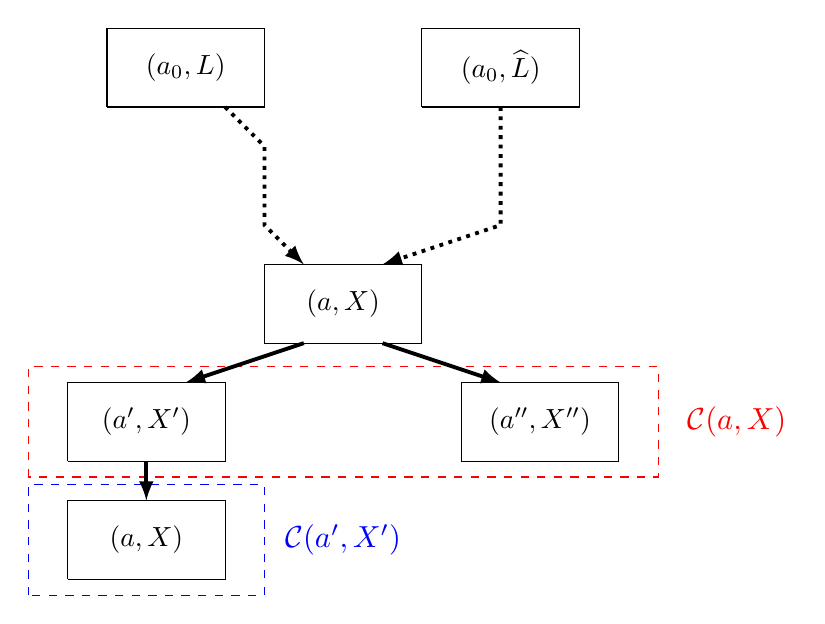
\begin{tikzpicture}


% RED BLOCKS %%%%%%%%%%%%%%%%%%%%%%

\draw [color = red, dashed] (1.0,4.8) -- (1.0,6.2) -- (9
.0,6.2) -- (9.0,4.8) -- (1.0,4.8);
\draw [color = blue, dashed] (1.0,3.3) -- (1.0,4.7) -- (4
.0,4.7) -- (4.0,3.3) -- (1.0,3.3);

% BLOCS %%%%%%%%%%%%%%%%%%%%%%%%%%%%%%%%%%%%%%%%%%%%%%%%%%%%%%%%%%%%%%%%%%

\draw [color = black, fill = white] (6.0,9.5) -- (6.0,10.5) -- (8.0,10.5) -- (8.0,9.5) --  (6.0,9.5);
\draw [color = black, fill = white] (2.0,9.5) -- (2.0,10.5) -- (4.0,10.5) -- (4.0,9.5) --  (2.0,9.5);
\draw [color = black, fill = white] (4.0,6.5) -- (4.0,7.5) -- (6.0,7.5) -- (6.0,6.5) -- (4.0,6.5);
\draw [color = black, fill = white] (1.5,5.0) -- (1.5,6.0) -- (3.5,6.0) -- (3.5,5.0) -- (1.5,5.0);
\draw [color = black, fill = white] (6.5,5.0) -- (6.5,6.0) -- (8.5,6.0) -- (8.5,5.0) -- (6.5,5.0);
\draw [color = black, fill = white] (1.5,3.5) -- (1.5,4.5) -- (3.5,4.5) -- (3.5,3.5) -- (1.5,3.5);

% CUBES

\node (P1) at (3.0,10.0) {$(a_0,L)$};
\node (P1') at (7.0,10.0) {$(a_0,\widehat{L})$};
\node (P2) at (5.0,7.0) {$(a,X)$};
\node (P3) at (2.5,5.5) {$(a',X')$};
\node (P4) at (7.5,5.5) {$(a'',X'')$};
\node (P5) at (2.5,4.0) {$(\Tilde{a},\Tilde{X})$};


% ETIQUETTES

\node[scale=1.1, color = red] at (10.0,5.5) {$\mathcal{C}(a,X)$};
\node[scale=1.1, color = blue] at (5.0,4.0) {$\mathcal{C}(a',X')$};

% LINKS %%%%%%%%%%%%%%%%%%%%%%%%%%%%%%%%%%%%%%%%%%%%%%%%%%%%%%%%%%%%%%%%%%

\draw[->,>=latex,line width = 1.4pt] (4.5,6.5)--(3.0,6.0);
\draw[->,>=latex,line width = 1.4pt] (5.5,6.5)--(7.0,6.0);
\draw[->,>=latex,line width = 1.4pt] (2.5,5.0)--(2.5,4.5);
%\draw[->,>=latex,line width = 2pt, color=blue] (13.2,12.0)--(13.2,4.0);

\draw[->,>=latex,dotted,line width = 1.4pt] (7.0,9.5) -- (7.0,8.0) -- (5.5,7.5);
\draw[->,>=latex,dotted,line width = 1.4pt] (3.5,9.5) -- (4.0,9.0) -- (4.0,8.0) -- (4.5,7.5);


\end{tikzpicture}
